\documentclass[UTF8,a4paper,12pt]{ctexart}
\usepackage{amsmath,amssymb,booktabs,graphicx,float,geometry}
\geometry{left=2.5cm,right=2.5cm,top=2.6cm,bottom=2.6cm}
\graphicspath{{../figures/}}
\title{2020年全国大学生数学建模竞赛B题第一问结果图表稿}
\author{}
\date{}

\begin{document}
\maketitle

\section{第一问模型与求解结果}

第一问被建模为有限期资源约束状态模型，并等价展开为逐日整数网络流。模型以日期、位置、水和食物为状态，以现金为价值，统一表示行走、停留、挖矿和村庄补给。两关均由 HiGHS 求得零 MIP 间隙的全局最优解，并由独立规则引擎逐日复算。第一关最优终端财富为10470元，于第24天到达终点；第二关最优终端财富为12730元，于第30天到达终点。

\begin{figure}[H]
  \centering
  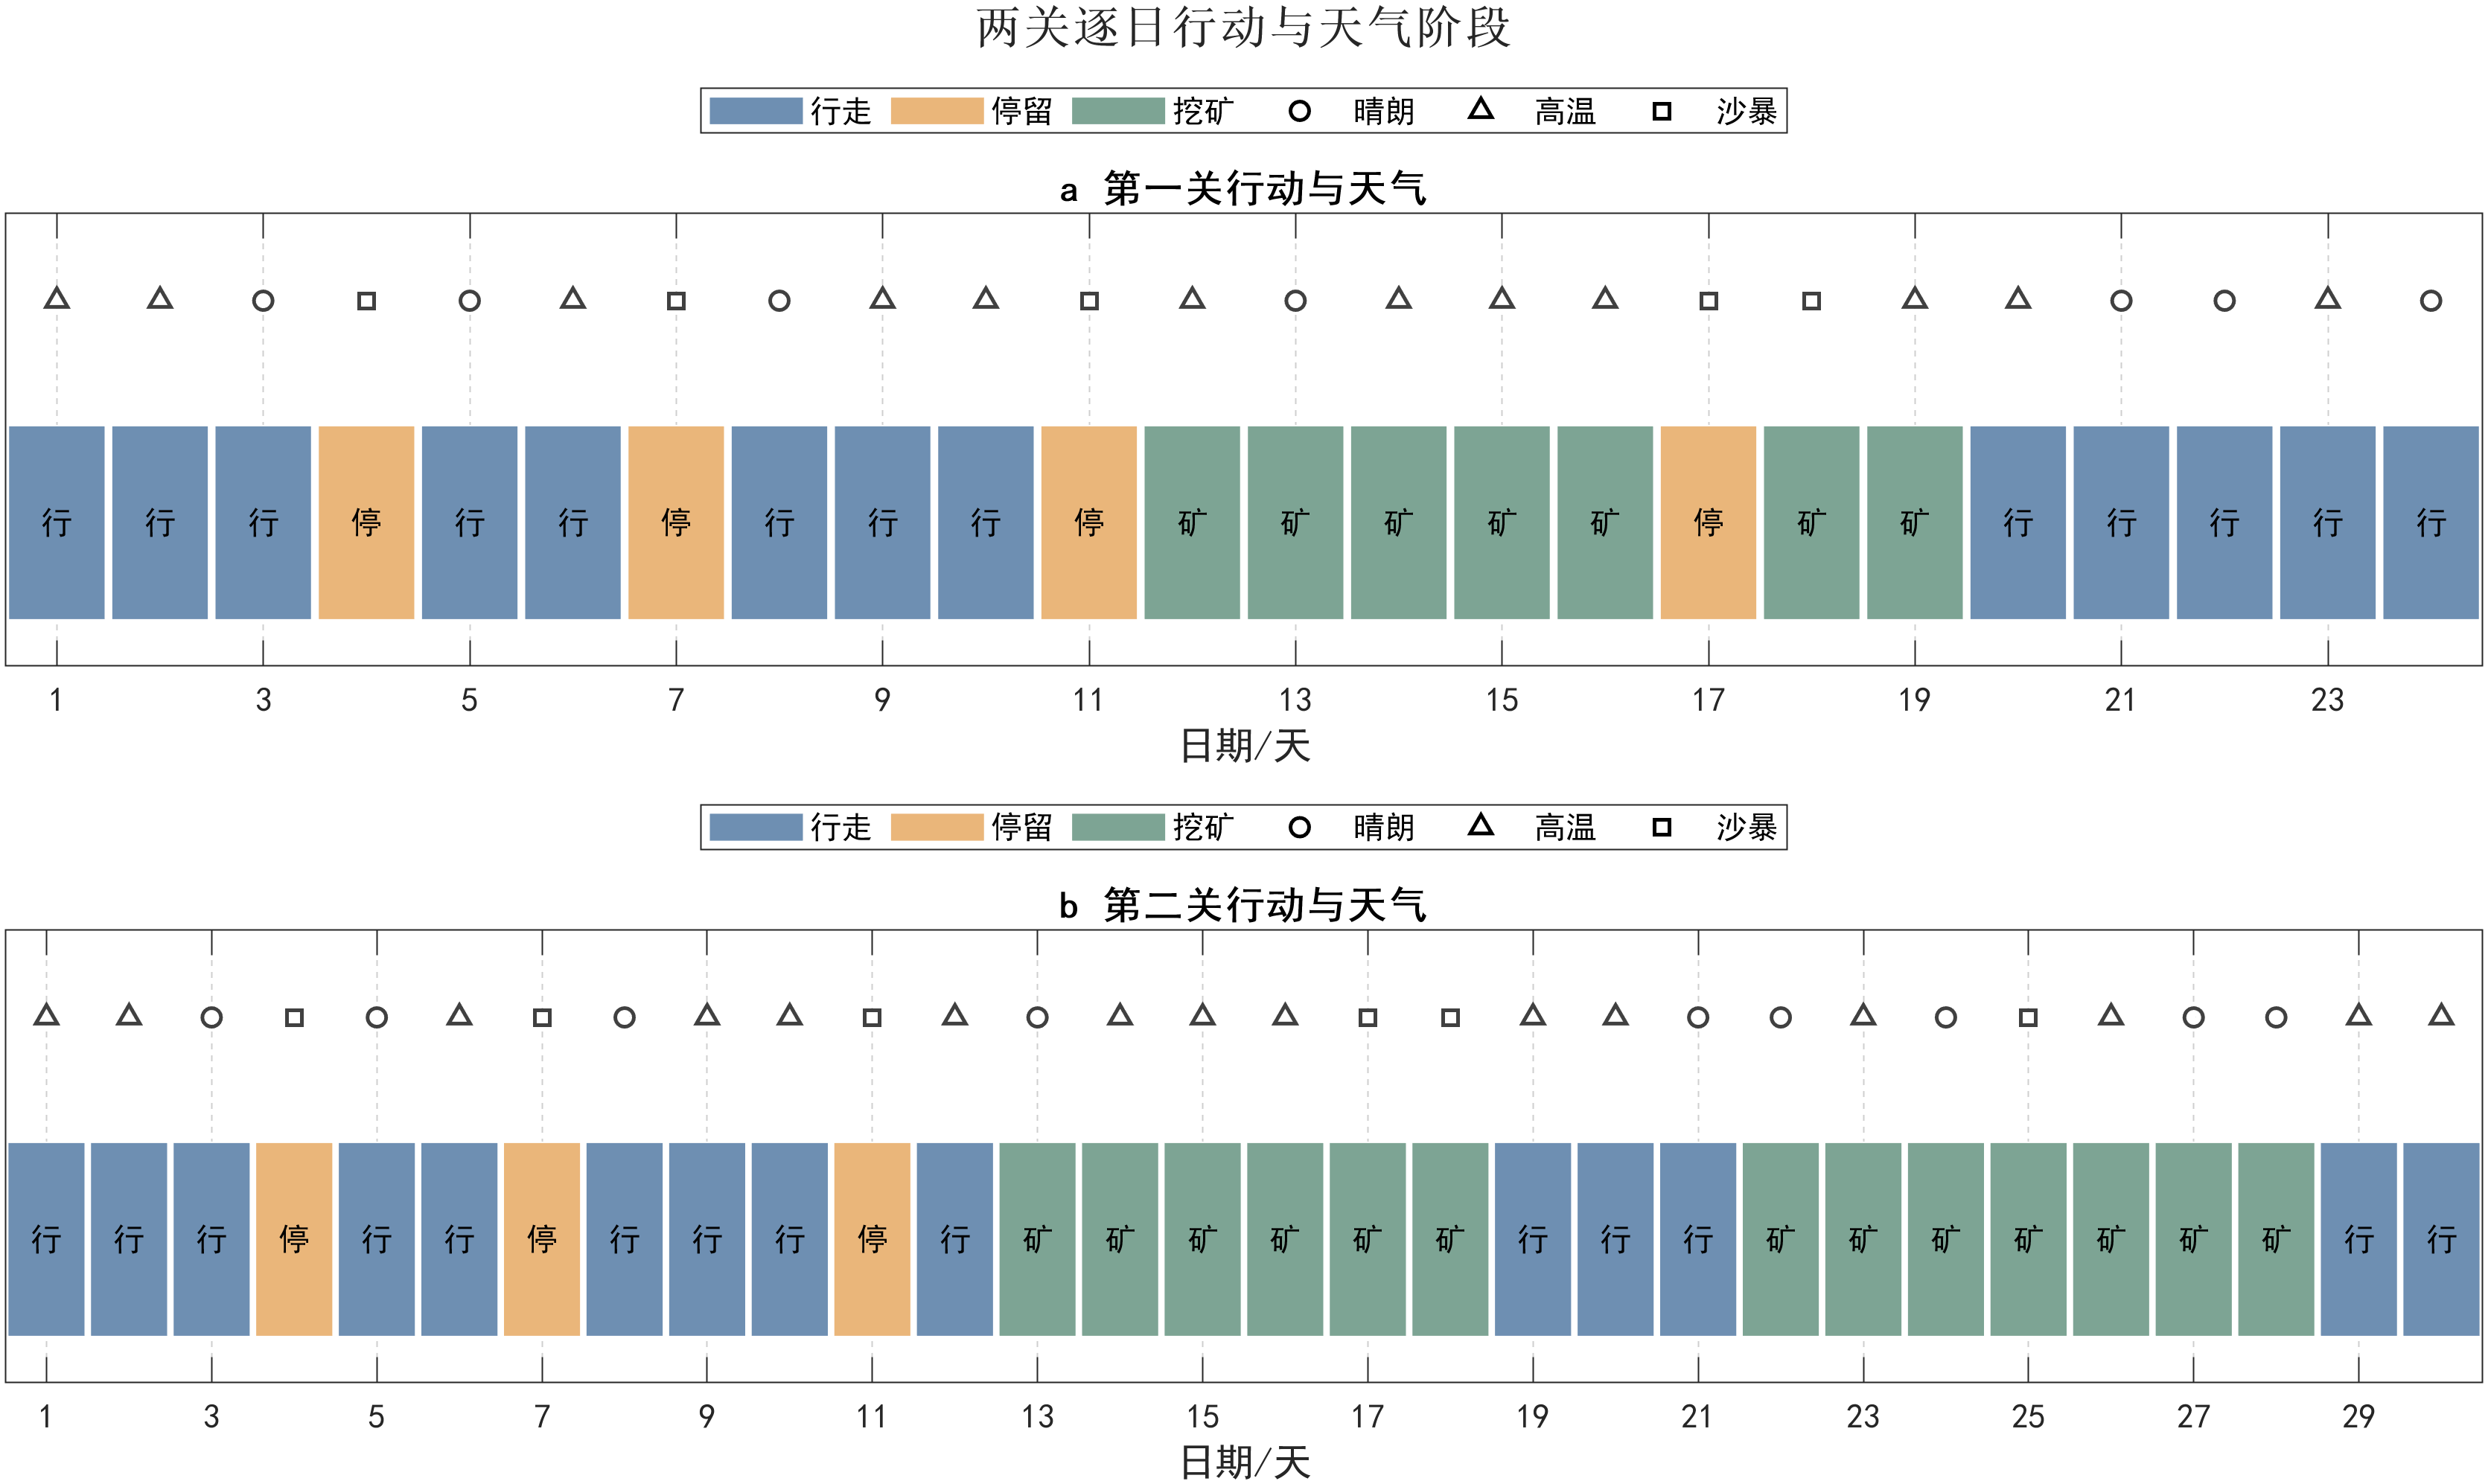
\includegraphics[width=0.98\textwidth]{fig_q1_strategy_timeline.png}
  \caption{两关逐日行动与天气阶段}
\end{figure}

由图1可见，最优策略并非机械遵循最短路径，而是依据已知天气在移动、停留和挖矿之间逐日切换。第一关收益行为集中在单一矿山，第二关则形成两段矿山作业期，说明地图功能节点与剩余时间共同决定收益安排。

\begin{figure}[H]
  \centering
  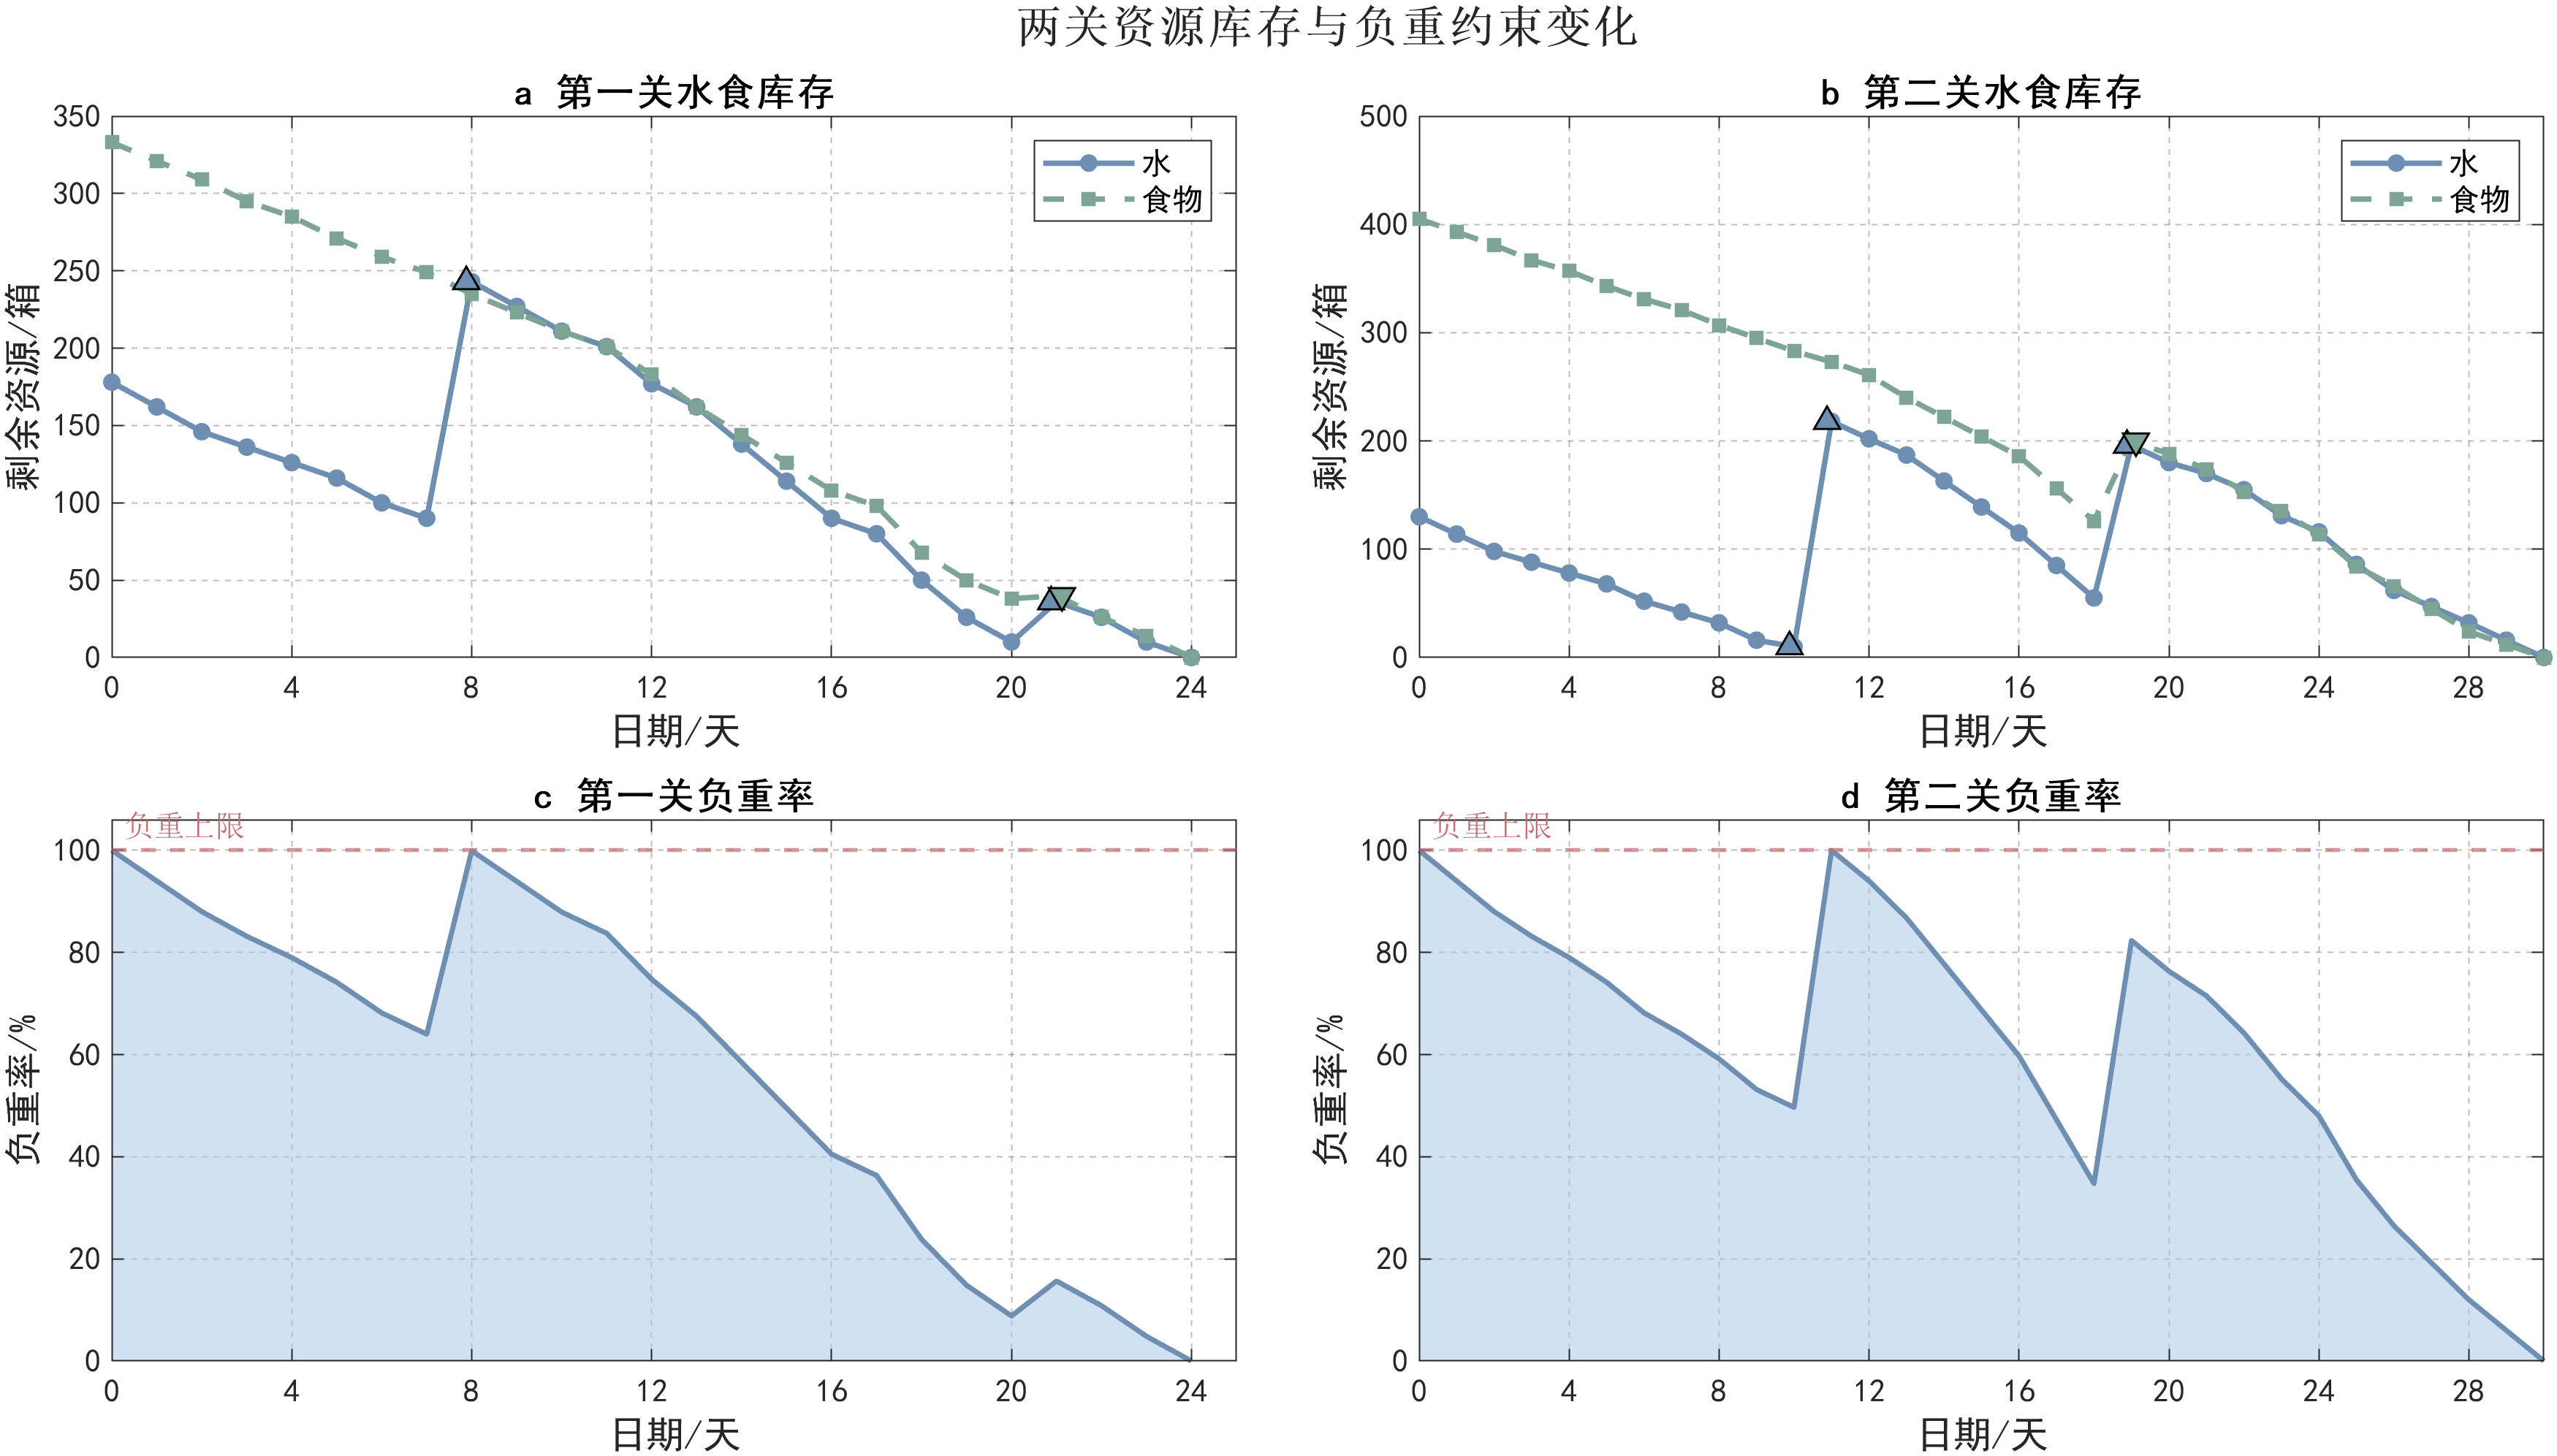
\includegraphics[width=0.98\textwidth]{fig_q1_resource_dashboard.png}
  \caption{两关资源库存与负重约束变化}
\end{figure}

图2表明，两关第0天均充分利用1200千克负重上限，随后在村庄按后续任务所需进行阶段性补给。库存跃升与负重率回升一一对应，且到达终点时水和食物均为0，说明末段补给与移动消耗实现精确匹配。

\begin{figure}[H]
  \centering
  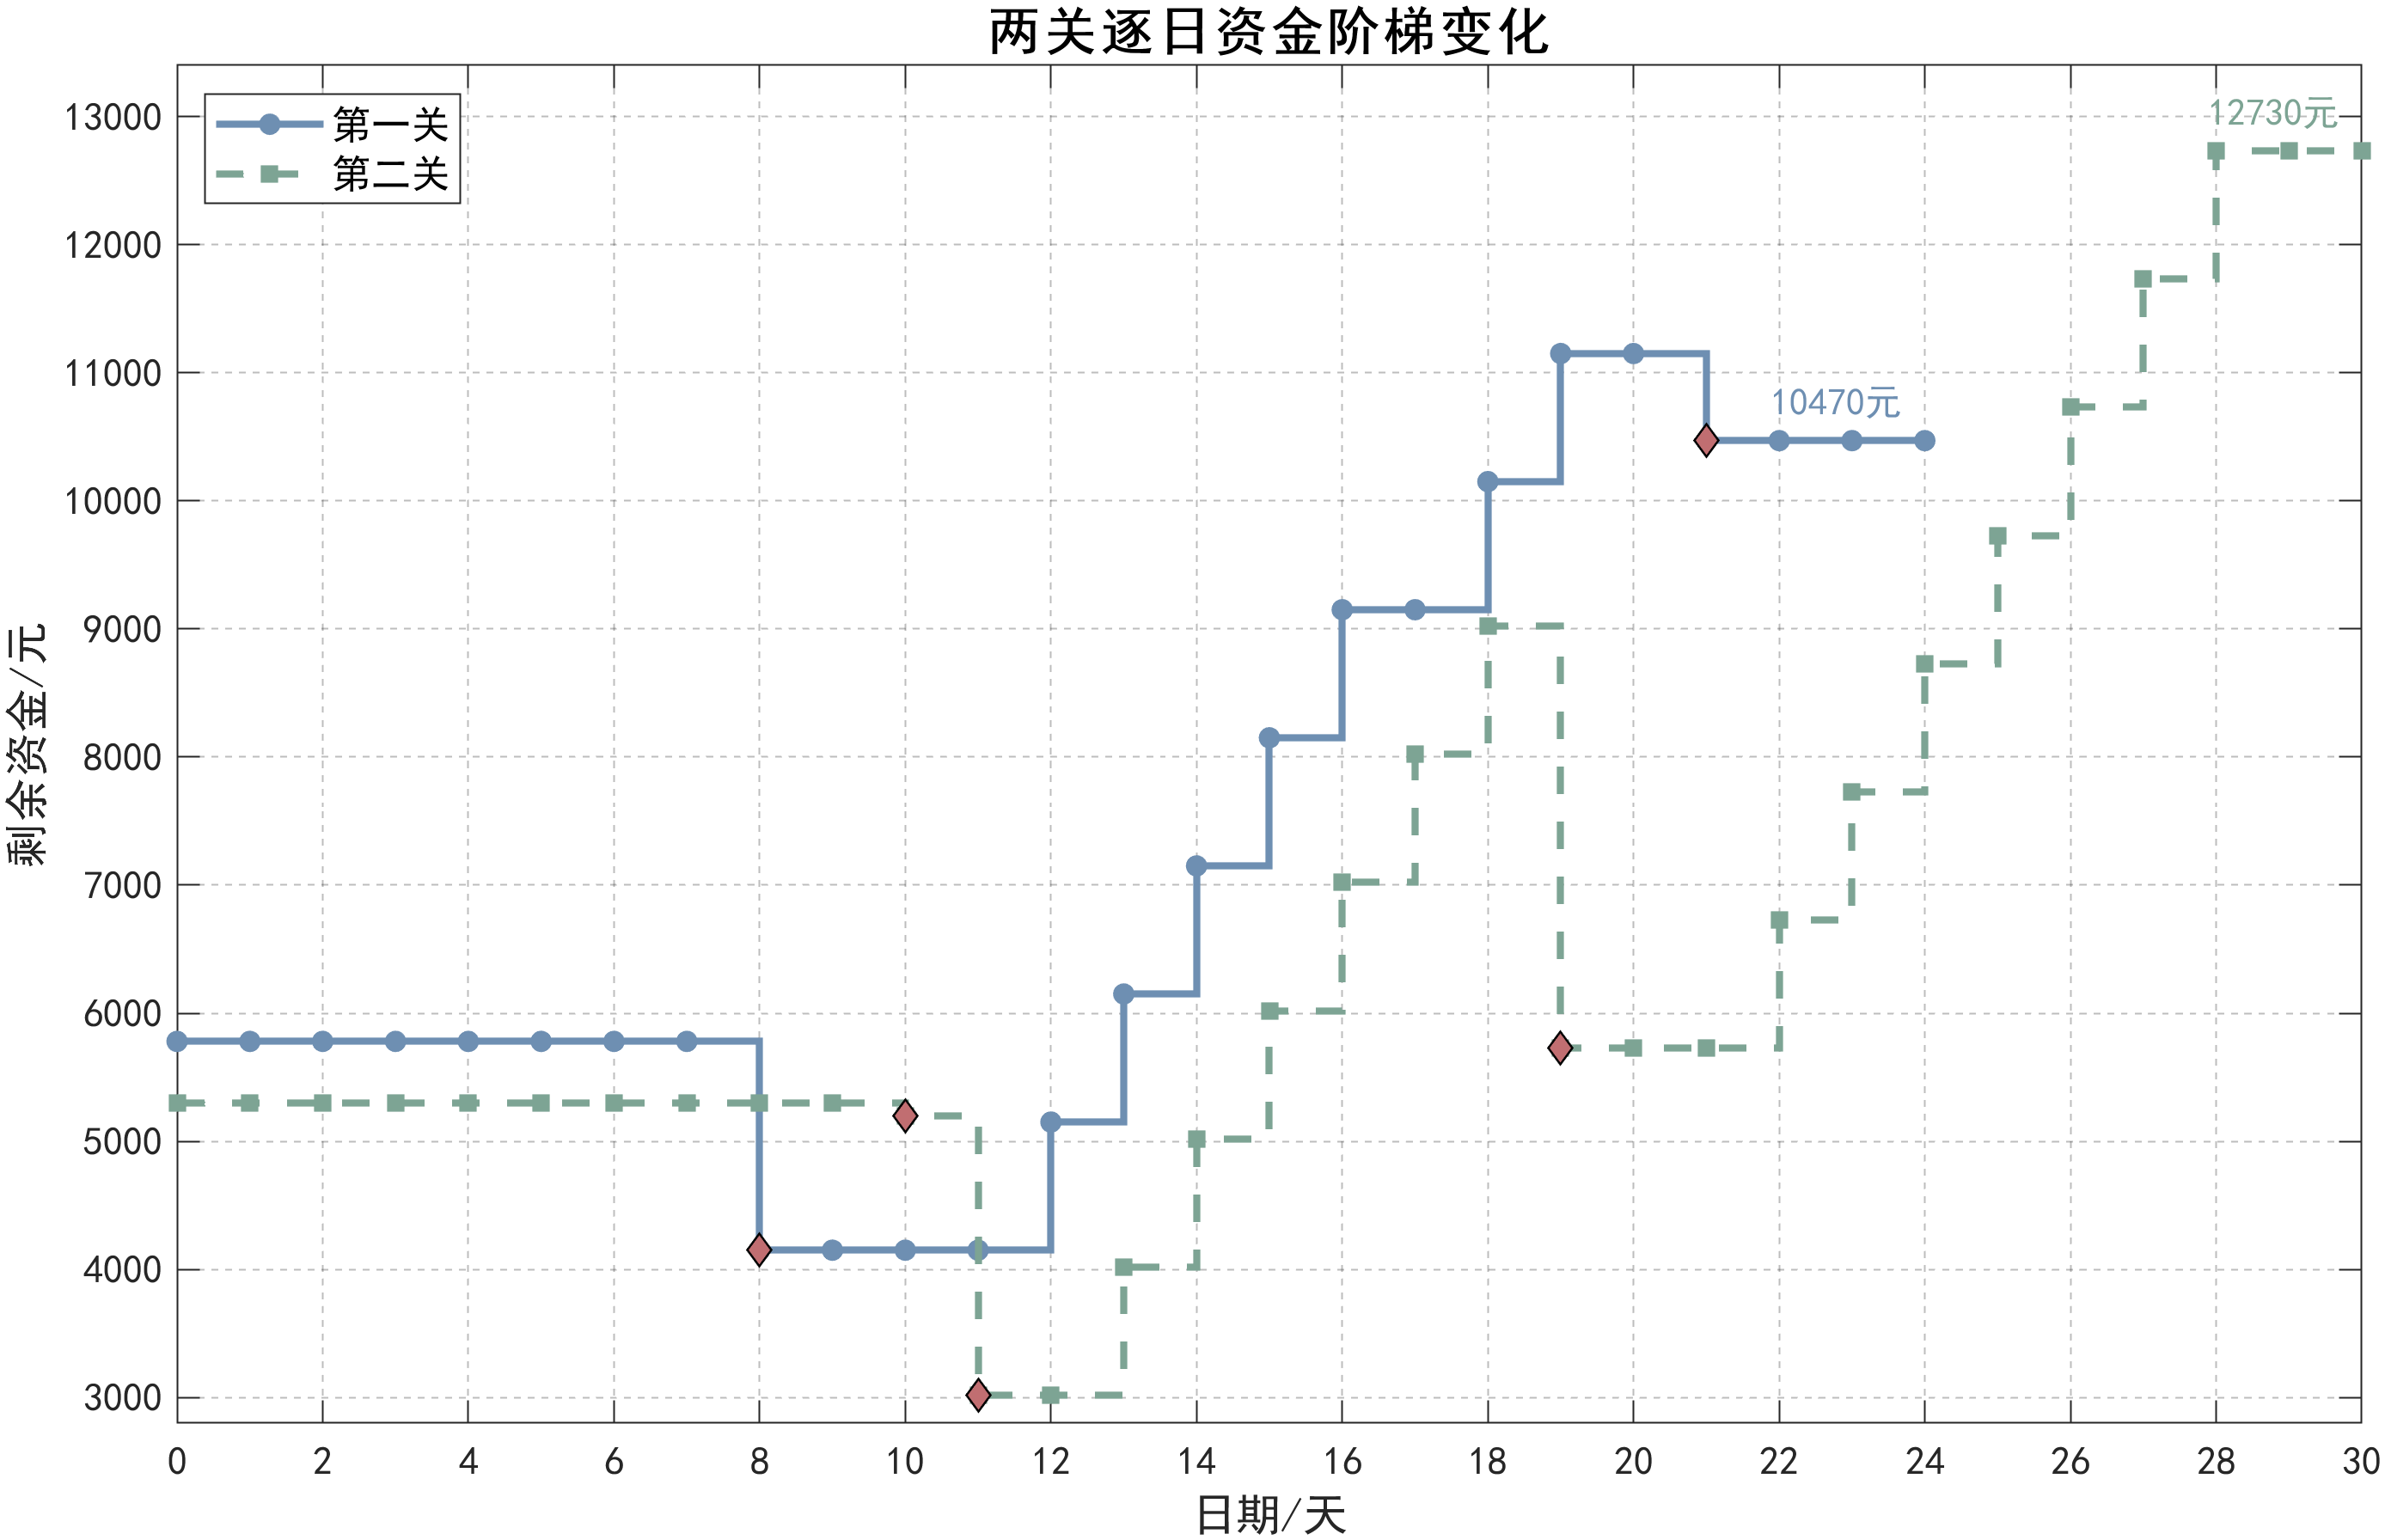
\includegraphics[width=0.94\textwidth]{fig_q1_cash_stairs.png}
  \caption{两关逐日资金阶梯变化}
\end{figure}

如图3所示，资金轨迹呈现采购下降、挖矿上升、再次补给和终点结算的阶梯结构。第二关虽然村庄补给成本更高，但两个矿山阶段带来的累计收益覆盖了补给支出，使其终端财富高于第一关。

\begin{figure}[H]
  \centering
  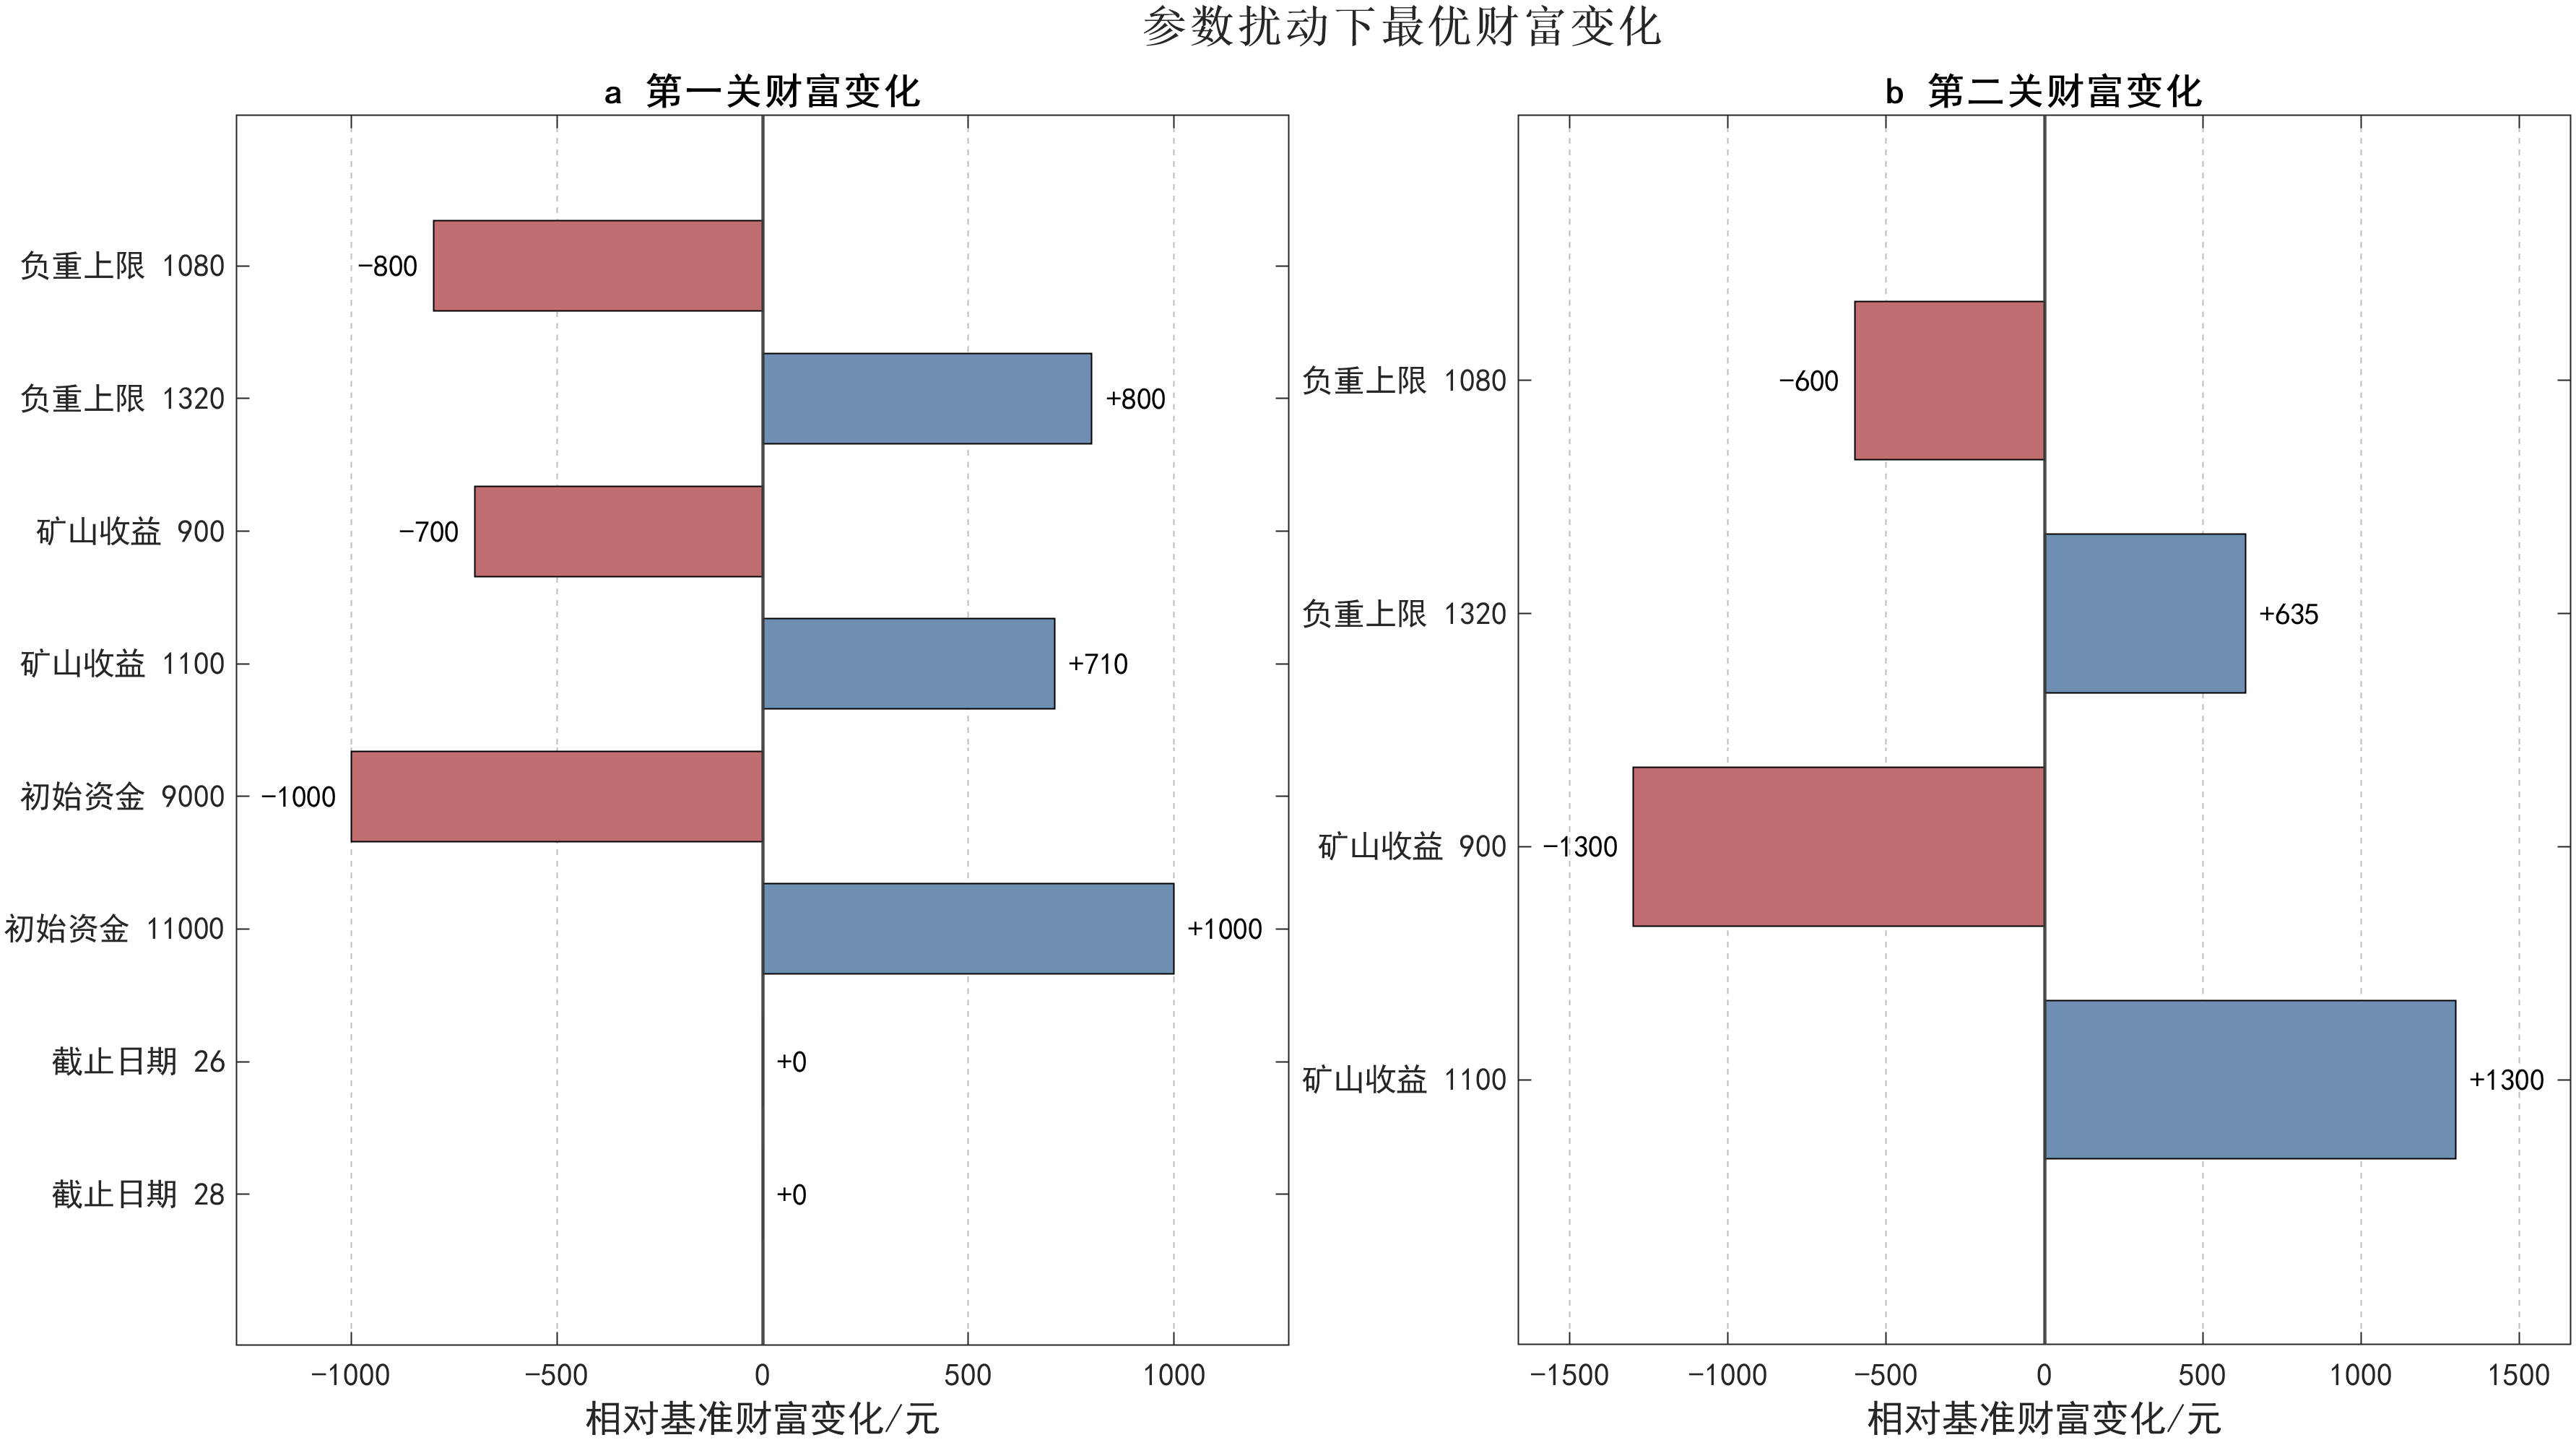
\includegraphics[width=0.98\textwidth]{fig_q1_sensitivity_diverging.png}
  \caption{参数扰动下最优财富变化}
\end{figure}

图4说明负重与矿山收益均为正向驱动因素，但影响强度受最优挖矿天数和补给结构制约。第二关具有13个有效挖矿日，因此矿山收益每变化100元，最优财富相应变化1300元；第一关在截止日26至30天范围内最优财富不变，反映第24天到达方案具有时间裕度。

\section{可靠性与适用边界}

两关逐日策略均满足邻接、沙暴禁行、资源非负、负重不超限、现金非负、村庄采购和终点吸收约束。灵敏性图只使用完整整数模型实际重求解的参数点，不对未计算区间进行插值。模型依赖全时段天气完全已知，不能直接替代未知天气下的在线决策模型。

\end{document}
